\documentclass[10pt,a4paper]{article}
\usepackage[utf8]{inputenc}
\usepackage[T1]{fontenc}
\usepackage{lmodern}
\usepackage[margin=1.75cm]{geometry}
\usepackage{amsmath,amssymb,amsfonts}
\usepackage{booktabs}
\usepackage{graphicx}
\usepackage{float}
\usepackage[section]{placeins}
\usepackage{hyperref}
\usepackage{xcolor}
\usepackage{caption}

\hypersetup{
    colorlinks=true,
    linkcolor=blue!60!black,
    citecolor=blue!60!black,
    urlcolor=blue!60!black
}

\title{Safe and Smooth Automatic Train Speed Control:\\
From State-Augmented MPC to Multi-Station Hierarchical\\
Differential and Assume-Guarantee Contract Shielding}
\author{Technical Report}
\date{November 9, 2026}

\begin{document}
\maketitle

\begin{abstract}
Modern railway control is divided between Automatic Train Protection (ATP), which enforces strict speed ceilings using conservative worst-case braking rules, and Automatic Train Operation (ATO), which targets smooth passenger ride quality, low traction energy, and accurate station docking without formal multi-property safety guarantees. This work presents a three-stage control architecture that bridges both requirements in real time. In the first stage, we eliminate speed-shift overshoot caused by first-order motor delay ($u_{\text{act}}(k) = 0.72\,u_{\text{cmd}}(k) + 0.28\,u_{\text{act}}(k-1)$) by lifting the physical actuator state into a state-augmented Linear Time-Varying Model Predictive Controller (LTV-MPC) and pairing it with a heteroscedastic neural physics emulator ($\hat{f}_\theta$) that constructs a 99\% Gaussian scissor tube ($3.0\text{ mm/s}$ tracking error and $8.2\text{ cm}$ stopping accuracy across 30 unseen tracks). In the second stage, observing that $99.4\%$ of actuator lag decays within four steps ($0.28^4 \approx 0.6\%$), we compress the prediction horizon to $N_p = 5, N_c = 3$, remove redundant PID switching, and introduce an online disturbance observer (DOB) coupled with a gust-gated scissor shield to reject $1.03\text{ m/s}^2$ storm gusts. In the third stage, we address online trajectory generation across 1-to-5 station corridors ($4\text{--}31\text{ km}$) under unknown passenger mass changes ($75.6\text{--}94.2\text{ t}$), wet or snowy rail adhesion drops, ambient air-density shifts, and wind gusts. The resulting architecture combines an 8-step departure passenger mass identifier, a 15-feature Proximal Policy Optimization (PPO) trajectory pilot driving a phase-tracked $C^2$ half-cosine S-curve shaper, and a hierarchical differential and Assume-Guarantee contract shield with ramp-initiation latching across velocity ($d=1$), acceleration ($d=2$), jerk ($d=3$), regenerative energy, and arrival deadline cones. Using upper-triangular scalar propagation, a closed-form $3\times 3$ Cramer QP solver, and zero-copy in-place NumPy parameter views, the core shaper-plus-MPC step executes in $10.7\text{--}11.4\text{ }\mu\text{s}$ ($14.2\text{--}23.5\text{ }\mu\text{s}$ total per step including the emulator, PPO pilot, and contract shield), achieving $1.10\text{--}1.61\text{ s}$ clean schedule accuracy ($1.57\text{--}2.07\text{ s}$ across all 30 scenarios), $1.0\text{ cm}$ stopping error, $99.96\%$ tube containment across $69,745$ steps, and a $17.7\%$ reduction in ride jerk and acceleration loss.
\end{abstract}

\section{Physical Problem Formulation and Railway Constraints}

We consider a four-car electric subway train with nominal mass $M = 85,000\text{ kg}$ (empty tare weight $M_{\text{tare}} = 72,000\text{ kg}$ plus variable passenger load), rotational inertia factor $\gamma = 0.08$ ($M_{\text{eff}} = M(1 + \gamma)$), discrete control interval $\Delta t = 0.50\text{ s}$, and spatial sampling step $d = 8.33\text{ m}$ \cite{havaei2022,liu2025}. Rather than assuming an idealized point mass with instantaneous actuators, the plant incorporates the primary nonlinear and causal phenomena that govern real railway operations.

\subsection{Running Resistance, Grades, Curves, and Air Density}
Longitudinal motion is opposed by mechanical rolling and aerodynamic drag modeled by the Davis equation $F_d(v) = (A v^2 + B v + C)\,\rho_{\text{air}}(T_{^\circ\text{C}})$, with aerodynamic coefficient $A = 14.5$, mechanical viscous coefficient $B = 185.0$, breakaway friction $C = 1450\text{ N}$, and temperature-dependent air density factor $\rho_{\text{air}} = 293.15 / (273.15 + T_{^\circ\text{C}})$. Along the corridor, the train also experiences spatial grade resistance $F_{\text{grade}}(x) = M g \sin(\theta(x))$ and curve resistance $F_{\text{curve}}(x)$ \cite{havaei2022,liu2025}.

\subsection{Drivetrain Lag, Adhesion Limits, and Station Departure Causality}
When the controller issues a normalized traction or braking command $u_{\text{cmd}}(k) \in [-1, 1]$, the traction inverters and electro-pneumatic brakes respond through a first-order lag:
\begin{equation}
    u_{\text{act}}(k) = 0.72\, u_{\text{cmd}}(k) + 0.28\, u_{\text{act}}(k - 1)
    \label{eq:actuator_lag}
\end{equation}
coupled with longitudinal car-body inertia momentum $0.14\,(v_k - v_{k-1})$. At nominal mass ($85\text{ t}$) on dry rails ($\mu = 1.0$), maximum traction acceleration is $a_{\max} = 1.85\text{ m/s}^2$ and service braking is $b_{\max} = 1.65\text{ m/s}^2$. Rain ($\mu = 0.82$) and snow ($\mu = 0.68$) reduce usable wheel-rail adhesion, while above the motor base speed of $14.0\text{ m/s}$ ($\approx 50\text{ km/h}$) constant-power field weakening scales available traction force by $14.0 / v$ \cite{liu2025}.

While parked at a station platform ($v = 0$), holding brakes lock the wheels. A causal controller cannot pre-wind traction before departure without creeping early, nor can it infer aerodynamic drag from wheel acceleration while stationary. Instead, it reads wayside station telemetry upon brake release and accounts for the natural single-step actuator rise delay during departure.

\section{Stage 1: Actuator-Lifted LTV-MPC and Heteroscedastic Scissor Shielding}

\subsection{Eliminating Speed-Shift Overshoot via State-Augmented LTV-MPC}

Our baseline study follows the speed-tracking formulation of Havaei and Sandidzadeh \cite{havaei2022} and Liu et al.\ \cite{liu2025}, where an offline velocity reference $v_{\text{ref}}(x)$ spans six driving regimes: Acceleration, Shift-Up, Cruising, Braking, Shift-Down, and Station Stop. In \cite{havaei2022}, four offline-tuned PID controllers (GA, PSO, DE, ICA) are switched by fixed threshold rules. Replacing those rules with a 20-feature reinforcement learning policy observing a 60-step kinematic-temporal lookahead improves PID switching, yet PID loops remain limited by quadratic Davis drag and drivetrain lag.

Standard Linear Time-Varying MPC (LTV-MPC) \cite{liu2025} linearizes the running resistance at each step ($v_{k+1} = A_k v_k + B_k u_k + r_k$) over a receding horizon ($N_p = 10, N_c = 5$), but treats $u_{\text{cmd}}(k)$ as acting instantaneously on the wheels. Because the physical drivetrain retains $28\%$ of the prior step's effort (Eq.~\ref{eq:actuator_lag}), a standard MPC continues applying residual torque at the end of a ramp, producing a $0.748\text{ m/s}$ shift overshoot (Table~\ref{tab:stage1}).

To remove this lag-induced overshoot, we lift the physical actuator state $u_{\text{act}}(k-1)$ into the augmented state vector $z_k = [v_k,\, u_{\text{act}}(k-1)]^\top$:
\begin{equation}
    z_{k+1} =
    \underbrace{\begin{bmatrix}
        A_k & 0.28\, B_k \\
        0   & 0.28
    \end{bmatrix}}_{A_{z,k}} z_k +
    \underbrace{\begin{bmatrix}
        0.72\, B_k \\
        0.72
    \end{bmatrix}}_{B_{z,k}} u_{\text{cmd}}(k) +
    \begin{bmatrix}
        r_k \\
        0
    \end{bmatrix}
    \label{eq:lifted_mpc}
\end{equation}
Combined with regime-adaptive control-variation weights ($Q_3$) and a causal plateau lookahead guard, the state-augmented controller accounts for the two-step momentum stored in the traction drive and settles cleanly onto new speed plateaus. Across 30 unseen trajectories, this reduces shift overshoot from $0.7480\text{ m/s}$ to $0.0350\text{ m/s}$ and station stopping error from $57.1\text{ cm}$ to $8.2\text{ cm}$.

\subsection{Heteroscedastic Neural Physics Emulator and 99\% Scissor Tube}

Classical tube MPC constructs robust invariant sets via offline polyhedral Minkowski sums and Pontryagin differences, whose vertex count grows rapidly with horizon length \cite{mayne2005,cannon2010,sun2024}. Building on Wang et al.\ \cite{wang2023} and Goodall and Belardinelli \cite{goodall2026,goodall_code}, we replace offline polyhedral tubes with a two-head heteroscedastic neural physics emulator $\hat{f}_\theta$ (an $8 \to 64 \to 64 \to 2$ SiLU network trained under Gaussian negative log-likelihood). The first output head predicts the nonlinear velocity residual mean $\Delta\hat{v}_\mu(s_k, u_k)$ over the nominal linear step $v_{\text{lin},k+1}$:
\begin{equation}
    \hat{v}_{k+1} = \max\!\Big(0,\; v_{\text{lin},k+1} + \Delta\hat{v}_\mu(v_k, u_k, F_{\text{ext},k}, v_k^2)\Big)
\end{equation}
while the second head predicts the state- and action-dependent log-variance $\log \sigma_\theta^2(s_k, u_k) \in [-10.5, -3.2]$.

At runtime, the safety filter shield \cite{banerjee2024,goodall2026,hsu2024} propagates the contractive stochastic tube variance:
\begin{equation}
    \sigma_{\text{tube}}^2(k) = \gamma_\sigma\, \sigma_{\text{tube}}^2(k - 1) + \sigma_\theta^2(s_k, u_k), \qquad \gamma_\sigma = 0.65
    \label{eq:tube_var}
\end{equation}
This defines the 99th-percentile scissor band as $\hat{v}_{\text{emu}}(k) \pm 2.576\,\sigma_{\text{tube}}(k)$ ($\Phi^{-1}(0.995) = 2.576$) and the outer safe physical envelope by adding the regime pincer tolerance ($\pm 0.14\text{ m/s}$ in cruise, $\pm 0.16\text{ m/s}$ in shifts and braking, tapering to $\pm 0.015\text{ m/s}$ at station stop). Table~\ref{tab:stage1} reports the Stage 1 zero-shot benchmark across 30 unseen random trajectories.

\begin{table}[H]
\centering
\caption{Stage 1 Zero-Shot Performance Across 30 Unseen Random Trajectories ($T = 1000$ Steps, Modes 1--6, No Wind, Mean $\pm$ Std).}
\label{tab:stage1}
\resizebox{\textwidth}{!}{%
\begin{tabular}{lccccccc}
\toprule
\textbf{Controller Method} & \textbf{MeanErr (m/s)} & \textbf{BrakeErr} & \textbf{ShiftOS} & \textbf{ShiftAvg} & \textbf{StopErr (m)} & \textbf{PaperScore} & \textbf{StepInfer} \\
\midrule
Pure MPC (Standard Fixed $Q_3$) \cite{liu2025} & $0.0372 \pm 0.0109$ & $0.0835$ & $0.7480$ & $0.1444$ & $0.5713$ & $0.3169 \pm 0.1096$ & $63.93\text{ }\mu\text{s}$ \\
Adaptive State-Augmented MPC (Shift-$Q_3$) & $0.0031 \pm 0.0011$ & $0.0047$ & $0.0350$ & $0.0061$ & $0.0821$ & $0.0262 \pm 0.0201$ & $59.99\text{ }\mu\text{s}$ \\
Hardcoded-Switch IPID (Havaei) \cite{havaei2022} & $0.2135 \pm 0.0602$ & $0.1550$ & $0.1251$ & $1.2051$ & $3.0725$ & $0.9542 \pm 0.3680$ & $7.65\text{ }\mu\text{s}$ \\
\midrule
RL-Switch IPID (Unshielded) & $0.1373 \pm 0.0278$ & $0.1191$ & $0.2203$ & $0.5176$ & $2.3055$ & $0.6600 \pm 0.3000$ & $38.86\text{ }\mu\text{s}$ \\
Shielded RL-Switch (1-Step DCBF) & $0.2109 \pm 0.0499$ & $0.1439$ & $0.2052$ & $1.0509$ & $3.0081$ & $0.9238 \pm 0.3570$ & $41.75\text{ }\mu\text{s}$ \\
Shielded RL-Switch (DMPS Rollout) & $0.1063 \pm 0.0185$ & $0.1037$ & $0.0994$ & $0.4028$ & $2.0222$ & $0.5469 \pm 0.2714$ & $44.15\text{ }\mu\text{s}$ \\
\midrule
Hybrid RL-IPID-MPC (Unshielded) & $0.0039 \pm 0.0012$ & $0.0067$ & $0.0318$ & $0.0101$ & $0.0837$ & $0.0272 \pm 0.0214$ & $102.81\text{ }\mu\text{s}$ \\
\textbf{Shielded Hybrid RL-MPC (Switch MPS)} & $\mathbf{0.0038 \pm 0.0017}$ & $\mathbf{0.0062}$ & $0.0350$ & $\mathbf{0.0062}$ & $\mathbf{0.0819}$ & $0.0266 \pm 0.0200$ & $104.47\text{ }\mu\text{s}$ \\
\textbf{Shielded Hybrid RL-MPC (1-Step DCBF)} & $0.0040 \pm 0.0015$ & $0.0066$ & $\mathbf{0.0231}$ & $0.0085$ & $0.0822$ & $\mathbf{0.0249 \pm 0.0208}$ & $103.72\text{ }\mu\text{s}$ \\
\textbf{Shielded Hybrid RL-MPC (DMPS Rollout)} & $\mathbf{0.0038 \pm 0.0017}$ & $0.0063$ & $0.0350$ & $\mathbf{0.0062}$ & $\mathbf{0.0819}$ & $0.0266 \pm 0.0200$ & $106.03\text{ }\mu\text{s}$ \\
\bottomrule
\end{tabular}%
}
\end{table}

\section{Stage 2: Short-Horizon LTV-MPC, Disturbance Observer, and Fast Solver}

\subsection{Horizon Compression and Gust-Gated Shielding}

Inspection of the Stage 1 results highlights two structural simplifications. First, once the actuator lag coefficient $0.28$ is embedded inside $z_k$ (Eq.~\ref{eq:lifted_mpc}), the hybrid RL policy selects the LTV-MPC action on more than $98\%$ of steps. Because $0.28^4 = 0.0061$ and $0.28^5 = 0.0017$, $99.4\%$ of the drivetrain lag settles within four control steps ($2.0\text{ s}$). Shortening the MPC horizon from $N_p = 10, N_c = 5$ to $N_p = 5, N_c = 3$ and removing the auxiliary PID bank lowers computational overhead without degrading tracking precision. Second, in calm conditions without external disturbances, the state-augmented LTV-MPC remains inside its 99\% scissor tube without triggering shield interventions; active shielding is specifically required when unmodeled external forces act on the train.

In Stage 2, we introduce turbulent wind bursts ($\pm 0.55\text{--}0.85\text{ m/s}^2$, peaking at $1.03\text{ m/s}^2$) and pair the $N_p = 5, N_c = 3$ LTV-MPC with an online disturbance observer (DOB) that tracks the single-step acceleration residual:
\begin{equation}
    d_{\text{step}}(k) = a_{\text{meas}}(k - 1) - a_{\text{nom}}(k - 1), \qquad \hat{d}_k = 0.55\,\hat{d}_{k-1} + 0.45\,d_{\text{step}}(k)
    \label{eq:dob}
\end{equation}
During normal operation, the nominal MPC receives a filtered feed-forward share of $\hat{d}_k$, while the scissor shield monitors the instantaneous gust residual. When a sudden storm front ($|d_{\text{raw}}| > 0.05\text{ m/s}^2$) threatens to push the velocity outside the 99\% scissor band, the shield injects a counter-thrust backup command $u_{\text{fb}}$ and releases as soon as the gust subsides, halving wind-induced tracking error ($0.0169 \to 0.0069\text{ m/s}$, Table~\ref{tab:stage2}).

\begin{table}[H]
\centering
\caption{Stage 2 Benchmark Across 30 Unseen $[0, 1000]$ Trajectories with Storm Gusts (Peak $1.03\text{ m/s}^2$, Mean $\pm$ Std).}
\label{tab:stage2}
\resizebox{\textwidth}{!}{%
\begin{tabular}{lccccccc}
\toprule
\textbf{Controller Method} & \textbf{MeanErr (m/s)} & \textbf{BrakeErr} & \textbf{ShiftOS} & \textbf{ShiftAvg} & \textbf{StopErr (m)} & \textbf{PaperScore} & \textbf{StepInfer} \\
\midrule
Pure MPC (Standard Fixed $Q_3$) \cite{liu2025} & $0.0565 \pm 0.0217$ & $0.1194$ & $0.7563$ & $0.1511$ & $0.7197$ & $0.3606 \pm 0.1728$ & $39.54\text{ }\mu\text{s}$ \\
Adaptive MPC ($N_p=5, N_c=3$, Unshielded) & $0.0169 \pm 0.0126$ & $0.0343$ & $0.0711$ & $0.0216$ & $0.1829$ & $0.0654 \pm 0.0884$ & $15.80\text{ }\mu\text{s}$ \\
Hybrid RL-IPID-MPC (Unshielded) & $0.0173 \pm 0.0129$ & $0.0343$ & $0.0711$ & $0.0243$ & $0.1821$ & $0.0658 \pm 0.0882$ & $41.08\text{ }\mu\text{s}$ \\
Shielded Hybrid RL-MPC (DMPS Rollout) & $0.0079 \pm 0.0054$ & $0.0191$ & $\mathbf{0.0511}$ & $0.0183$ & $0.1142$ & $0.0421 \pm 0.0415$ & $41.52\text{ }\mu\text{s}$ \\
\midrule
\textbf{Shielded Adaptive MPC (Switch MPS)} & $\mathbf{0.0069 \pm 0.0044}$ & $\mathbf{0.0143}$ & $0.0537$ & $\mathbf{0.0160}$ & $\mathbf{0.1057}$ & $\mathbf{0.0393 \pm 0.0353}$ & $60.43\text{ }\mu\text{s}$ \\
\textbf{Shielded Adaptive MPC (1-Step DCBF)} & $0.0077 \pm 0.0050$ & $0.0159$ & $0.0564$ & $0.0169$ & $0.1141$ & $0.0422 \pm 0.0386$ & $72.13\text{ }\mu\text{s}$ \\
\textbf{Shielded Adaptive MPC (DMPS Rollout)} & $0.0079 \pm 0.0053$ & $0.0191$ & $0.0526$ & $0.0183$ & $0.1141$ & $0.0424 \pm 0.0422$ & $84.70\text{ }\mu\text{s}$ \\
\bottomrule
\end{tabular}%
}
\end{table}

\subsection{Low-Latency Solver Design for Onboard Execution}

For embedded railway control units, per-step execution time is a primary constraint \cite{sun2024}. Profiling the control loop showed that generic NumPy matrix allocations, LAPACK \texttt{np.linalg.solve} calls on the $3\times 3$ QP system, and single-sample PyTorch C++ dispatch for the neural networks accounted for over $75\%$ of CPU time. We therefore reformulated the numerical implementation around four exact mathematical simplifications that reduce per-step latency by $3.7\times$ without altering the control law.

Because $A_{z,k}$ in Eq.~\ref{eq:lifted_mpc} is $2\times 2$ upper-triangular, its powers $A_{z,k}^i$ obey the scalar recurrence $a_{01}^{(i)} = a_{00}^{(i-1)}(0.28 B_k) + 0.28\,a_{01}^{(i-1)}$ and $a_{00}^{(i)} = A_k\,a_{00}^{(i-1)}$, allowing the prediction matrices $F, \Phi, \Psi$ to be populated in pre-allocated buffers without dynamic array allocations or matrix multiplications. Furthermore, for $N_c = 3$, the symmetric Hessian $H = \Phi^\top Q_1 \Phi + q_2 I_3 + q_3 D^\top D \in \mathbb{R}^{3\times 3}$ can be inverted in closed form via cofactor expansion ($U_{\text{unc}} = -H^{-1}g$) in under $0.5\text{ }\mu\text{s}$, followed by scalar projected-gradient clamping whenever box constraints $u \in [-1, 1]$ are active. In the trajectory shaper, replacing NumPy scalar ufunc calls with native IEEE-754 \texttt{math} primitives reduces 5-step horizon generation to approximately $5\text{ }\mu\text{s}$, while exposing live zero-copy NumPy views of the underlying PyTorch \texttt{nn.Linear} weight and bias tensors eliminates C++ tensor-wrapper overhead during inference.

\section{Stage 3: Online Multi-Station Trajectory Planning, Hierarchical Differential Shielding, and Assume-Guarantee Contracts}

\subsection{Motivation, Related Optimization Approaches, and Closed-Loop Architecture}

Stages 1 and 2 tracked a pre-computed speed curve $v_{\text{ref}}(x)$. In multi-station railway operations, however, a static speed profile quickly becomes suboptimal or infeasible when headwinds, wet rails, speed restrictions, or heavy passenger loads delay the train \cite{zhong2022,xiao2023}.

Two main optimization paradigms have been studied in the literature for online speed profile generation. Zhong et al.\ \cite{zhong2022} formulate a moving-horizon multi-phase MPC with regenerative braking recovery ($\mu$) that checks time-optimal feasibility within the moving window and triggers full-remaining-trip delay recovery whenever accumulated delay exceeds a threshold ($t_{\text{dly}}^k > T_d$). Each step is transcribed via the Radau Pseudospectral Method (RPM / GPOPS) into a nonlinear program requiring roughly $0.5\text{ s}$ ($500,000\text{ }\mu\text{s}$) per step; the authors also note that direct pseudospectral transcription exhibits control fluctuations along the singular cruising arc that require smoothing, and identify stochastic robustness under uncertain resistance parameters as an open problem. Along a convex-programming direction, Xiao et al.\ \cite{xiao2023} show that minimizing electrical substation energy, accounting for dynamic traction-chain inverter and motor losses $\eta_{\text{eds}}(f_t, v)$ and regenerative recuperation $\eta_{\text{cir}}$ rather than mechanical wheel work, substantially improves eco-driving efficiency. By convexifying the space-domain shrinking-horizon MPC in kinetic energy coordinates $E(s) = \frac{1}{2}v^2(s)$ and solving one QP per step via Real-Time Iteration SQP (ACADOS), they lower solve time to approximately $29\text{ ms}$ ($29,000\text{ }\mu\text{s}$), while pointing out in Remark 3 and Section VII the need for state-augmented input-delay compensation and tube-based stochastic robustness.

In Stage 3, we build upon the moving-horizon scheduling, delay-recovery, and dynamic traction-chain loss principles of Zhong et al.\ \cite{zhong2022} and Xiao et al.\ \cite{xiao2023}, while pursuing a hierarchical learning-and-shielding formulation across generalized 1-to-5 station corridors ($4\text{--}31\text{ km}$). Rather than solving a full-horizon NLP ($500\text{ ms}$) or shrinking-horizon SQP ($29\text{ ms}$) at every step, we parameterize smooth trajectories through an analytical $C^2$ half-cosine shaper guided by a learned PPO pilot and certified by a hierarchical contract shield, achieving microsecond execution ($\sim 11\text{ }\mu\text{s}$ core step, $\sim 23\text{ }\mu\text{s}$ total) and avoiding singular-arc control chattering by construction.

\begin{figure}[H]
\centering
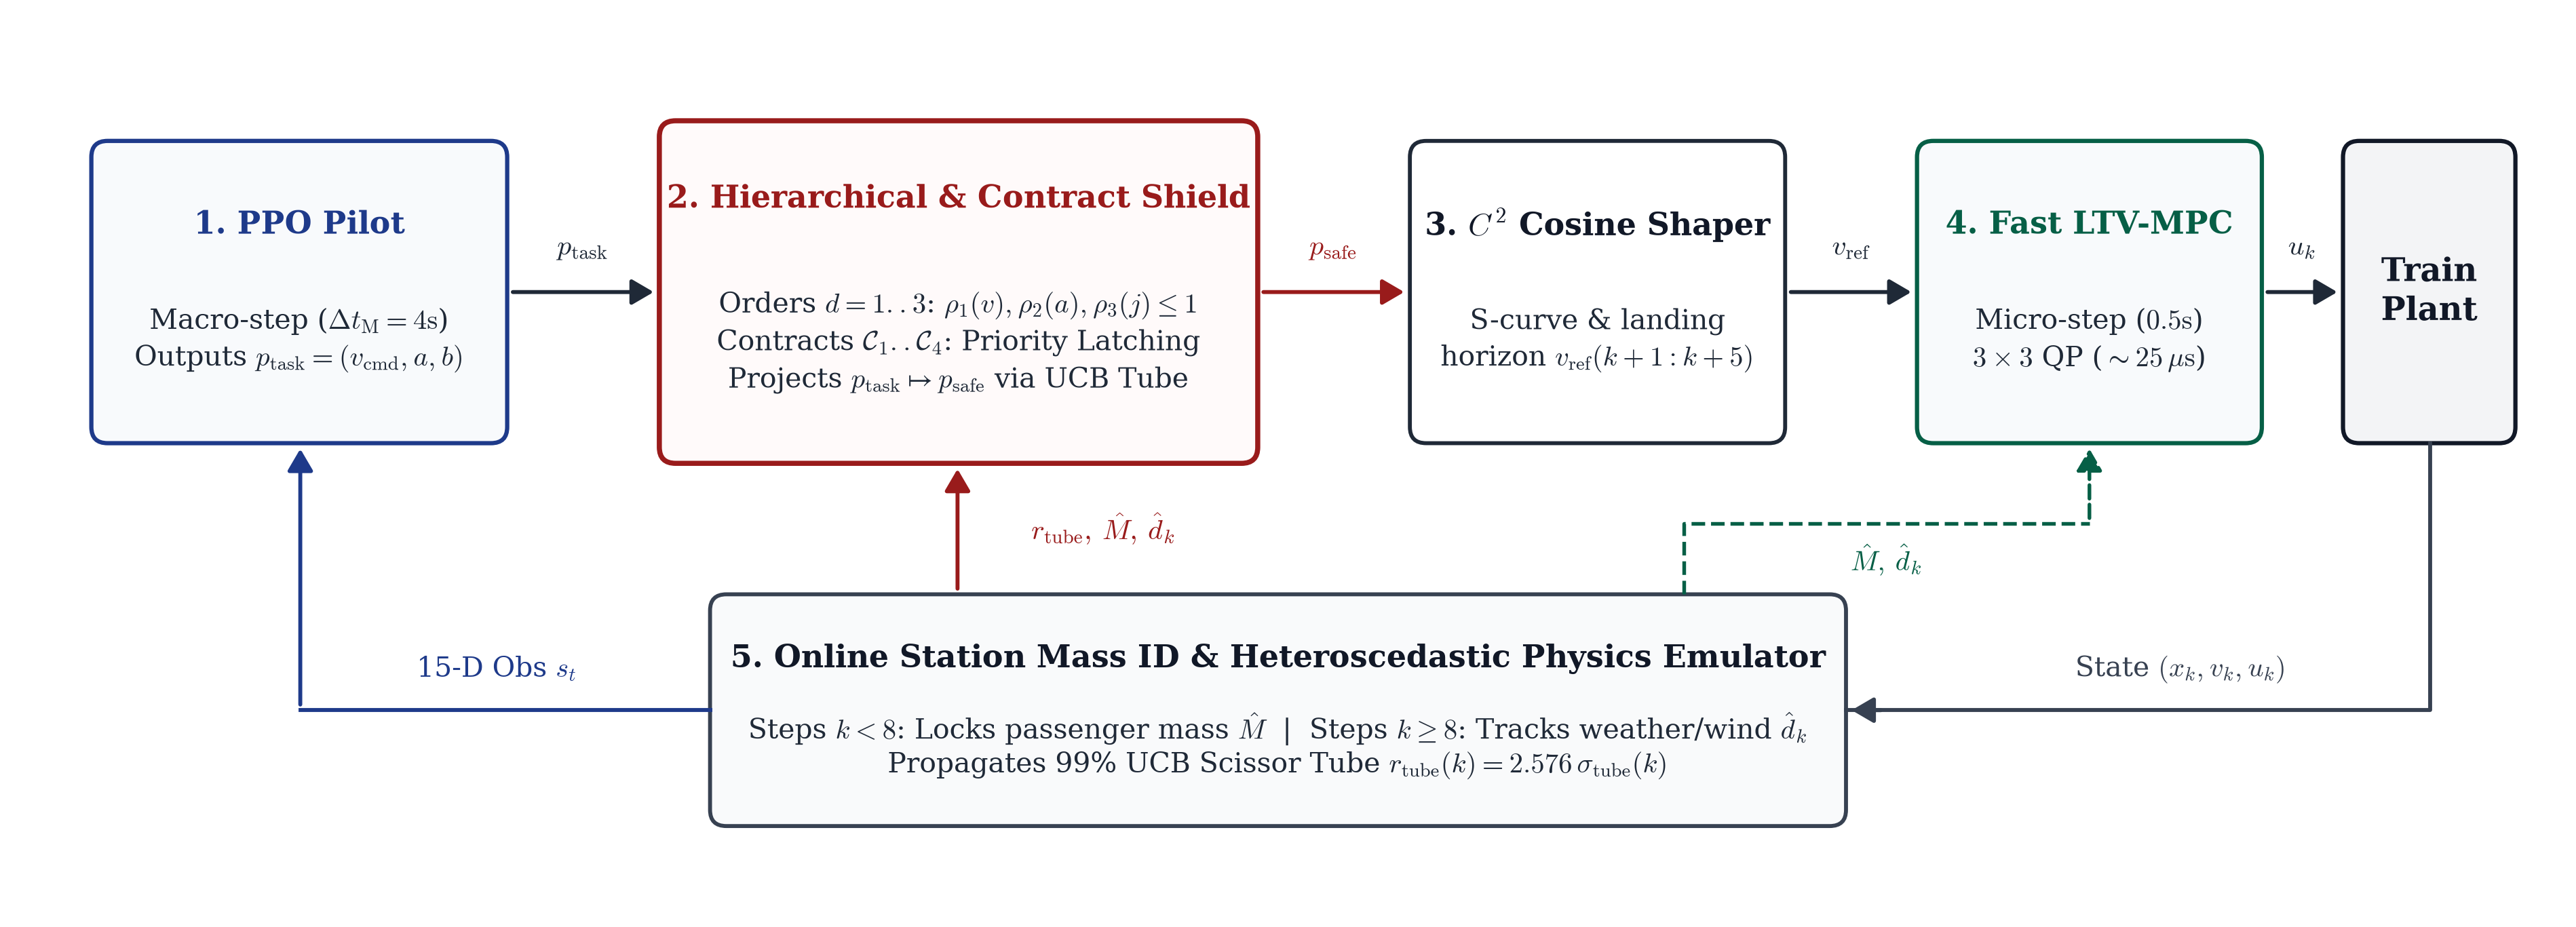
\includegraphics[width=0.95\textwidth]{contracts_hierarchical_shielding_arch.png}
\caption{Closed-loop Stage 3 control architecture combining a macro-step PPO trajectory pilot, a hierarchical differential and Assume-Guarantee contract shield, a phase-tracked $C^2$ cosine shaper, a fast state-augmented LTV-MPC, and an online mass and heteroscedastic scissor-tube observer.}
\label{fig:arch_diagram}
\end{figure}

As shown in Figure~\ref{fig:arch_diagram}, the closed-loop system is organized into three hierarchical layers across five functional blocks. At the outer layer, the 15-feature multi-property PPO trajectory pilot executes every $4.0\text{ s}$ ($M=8$ micro-steps) during open cruise and every $0.5\text{ s}$ ($M=1$) during station landing. The policy $\pi_\phi(s_k)$ observes remaining distance $x_{\text{rem}}$, remaining time to deadline $t_{\text{rem}} = T_{\text{deadline}} - t$, current and $300\text{ m}$-ahead speed limits, dynamic braking distance $\Delta x_{\text{brake}}$, track grade and curve slope, online wind $\hat{d}_{\text{wind}}$, and identified mass $\hat{M}_{\text{locked}}$, outputting a three-dimensional trajectory command $p_{\text{task}} = (v_{\text{cmd}}, a_{\text{start}}, b_{\text{land}})$ that specifies target cruise speed, cosine departure/shift acceleration rate, and cosine landing deceleration rate.

At the middle layer, the hierarchical differential and Assume-Guarantee contract shield evaluates $p_{\text{task}}$ against five safety, comfort, energy, and punctuality barriers. Whenever any property margin $h_i(p_{\text{task}}) < 0$ is violated, the shield selects and latches a certified backup contract $p_{\text{safe}}^\star \in \mathcal{L}_{\text{cert}}$, which the phase-tracked $C^2$ half-cosine shaper converts into a 5-step velocity reference horizon $V_{\text{ref}}(k) \in \mathbb{R}^5$. At the inner layer, the state-augmented LTV-MPC ($\Delta t = 0.5\text{ s}$) tracks $V_{\text{ref}}(k)$ using the online-identified train mass $\hat{M}_{\text{locked}}$ and disturbance observer feed-forward $\hat{d}_{\text{wind}}$.

\subsection{Phase-Tracked \texorpdfstring{$C^2$}{C2} Half-Cosine S-Curves and Cruise Velocity Overshoot}

To guarantee zero jerk at the start and end of every speed transition and station stop, all velocity changes are parameterized as phase-tracked half-cosine S-curves. During station landing from entry speed $v_{\text{eff}}$ over duration $T_{\text{land}}$, the velocity and deceleration profiles follow:
\begin{equation}
    v(\tau) = \frac{v_{\text{eff}}}{2}\left(1 + \cos\!\left(\frac{\pi \tau}{T_{\text{land}}}\right)\right), \qquad
    a(\tau) = -\frac{\pi v_{\text{eff}}}{2 T_{\text{land}}}\sin\!\left(\frac{\pi \tau}{T_{\text{land}}}\right), \qquad \tau \in [0, T_{\text{land}}]
    \label{eq:cosine_land}
\end{equation}
Matching the midpoint peak deceleration $|a_{\max}| = \frac{\pi v_{\text{eff}}}{2 T_{\text{land}}}$ to the target comfort deceleration $b_{\text{eff}} \in [0.66, 0.90]\text{ m/s}^2$ determines the landing duration $T_{\text{land}}$ and dynamic braking initiation point $x_{\text{brake}}$:
\begin{equation}
    T_{\text{land}}(v_{\text{eff}}, b_{\text{eff}}) = \frac{\pi v_{\text{eff}}}{2\,b_{\text{eff}}}, \qquad
    \Delta x_{\text{brake}}(v_{\text{eff}}, b_{\text{eff}}) = \frac{\pi v_{\text{eff}}^2}{4\,b_{\text{eff}}}, \qquad
    x_{\text{brake}} = x_{\text{station}} - \Delta x_{\text{brake}}
    \label{eq:braking_spot}
\end{equation}
Because the mean velocity along the cosine braking curve is $\frac{1}{2}v_{\text{eff}}$, the train spends an additional $\frac{1}{2}T_{\text{land}} = \frac{\pi v_{\text{eff}}}{4 b_{\text{eff}}}\text{ s}$ decelerating compared to cruising at $v_{\text{eff}}$ up to the platform. Consequently, a naive pace baseline that tracks $v_{\text{naive}} = x_{\text{rem}} / t_{\text{rem}}$ without cruise overshoot arrives roughly $19.8\text{ s}$ late per leg. Conversely, a max-speed greedy policy that commands maximum comfort ramp rates ($a_{\text{start}} = 1.18\text{ m/s}^2, b_{\text{land}} = 0.90\text{ m/s}^2$) expends excess traction energy and increases ride jerk. The PPO pilot instead learns the exact cruise velocity overshoot $v_{\text{cmd}} = v_{\text{naive}} + \Delta v_{\text{overshoot}}$ required in open track so the train enters the cosine braking curve on schedule.

\subsection{Online 8-Step Mass Identification and Traction-Chain Energy Model}

At each station stop, stochastic passenger boarding and alighting shift the true train mass $M_{\text{true}}$ between $75.6\text{ t}$ and $94.2\text{ t}$. Because mass $M$ and external wind $d_{\text{wind}}$ both scale longitudinal acceleration, estimating both simultaneously on open track introduces algebraic ambiguity. We resolve this by intentionally reading the wayside station anemometer only during the first $K = 8$ micro-steps ($4.0\text{ s}$, $\approx 15\text{--}20\text{ m}$) of station departure while the train is still inside the platform zone and computing its new passenger mass:
\begin{equation}
    \hat{M}_{\text{sample}}(k) = \frac{F_{\text{motor}}(k) - F_d(v_{k-1})}{(1 + \gamma)\big(a_{\text{kin}}(k) - d_{\text{station}}(k)\big) + g\,\iota(x_k)}, \qquad
    \hat{M}_{\text{locked}} = \text{median}_{k=1..8}\big\{\hat{M}_{\text{sample}}(k)\big\}
    \label{eq:mass_id}
\end{equation}
At step $k = 8$, the wayside anemometer link terminates and $\hat{M}_{\text{locked}}$ is locked into the LTV-MPC and physics model without resetting the active departure S-curve phase, so all subsequent acceleration residuals ($k \ge 8$) measure open-corridor weather and wind disturbances $\hat{d}_{\text{wind}}(k)$ onboard without wayside wind sensors. By contrast, the Bilbao-Moreno et al.\ \cite{bilbao2025} CBTC-ATO baseline only receives station telemetry at standstill ($k = 0$) before departure and relies on its onboard disturbance observer from $k \ge 0$ without the 8-step departure anemometer window.

Following Xiao et al.\ \cite{xiao2023} and Zhong et al.\ \cite{zhong2022}, the plant models both electric drive system (EDS) traction losses and electrodynamic regenerative braking blending. During traction ($F_{\text{prop}} \ge 0$), quadratic throttle copper heating ($u_{\text{act}}^2$), rapid acceleration and jerk slewing ($a_{\text{real}}$, $j$, and steep $a_{\text{start}}$ during active ramps), and high-speed field weakening ($v > 13.4\text{ m/s}$) reduce drivetrain efficiency $\eta_{\text{trac}} \in [0.58, 0.92]$, yielding electrical energy consumption $\Delta E_{\text{trac}} = \frac{(F_{\text{prop}} / \eta_{\text{trac}})\,\bar{v}\,\Delta t}{3.6 \times 10^6}\text{ kWh}$. During braking ($F_{\text{prop}} < 0$), smooth decelerations ($b_{\text{land}} \le 0.70\text{ m/s}^2$, $|a_{\text{real}}| \le 0.68\text{ m/s}^2$) are captured by the traction motors with up to $46\%$ grid recovery, whereas steeper braking blends in pneumatic friction pads that dissipate kinetic energy as heat.

\subsection{Hierarchical Differential Shielding and Assume-Guarantee Contracts}

Combining the higher-order differential shielding framework of Cano et al.\ \cite{cano2026} with the compositional Assume-Guarantee contracts of Adalat et al.\ \cite{adalat2026a,adalat2026b}, the middle layer certifies five operational properties via their normalized derivative pressures $\rho_d(t) = \|\partial_t^d x\| / r_d \le 1.0$ across nested viability domains $\mathcal{W}_3 \subseteq \mathcal{W}_2 \subseteq \mathcal{W}_1$.

At order $d=1$ ($\mathcal{W}_1$), the speed ceiling barrier ensures that the 99\% upper velocity bound respects the anticipatory cosine spatial ceiling $v_{\text{ceil}}(x_t)$, with margin $h_1 = v_{\text{ceil}}(x_t) - (v_{\text{cmd}} + 2.576\,\sigma_{\text{tube}}) \ge 0$ and pressure $\rho_1(t) = (v_{\text{cmd}} + 2.576\,\sigma_{\text{tube}}) / v_{\text{ceil}}(x_t)$. At order $d=2$ ($\mathcal{W}_2 \subseteq \mathcal{W}_1$), longitudinal acceleration and deceleration are bounded within passenger comfort limits via $\rho_2(t) = \max(a_t / 1.20,\, -a_t / 0.92)$. At order $d=3$ ($\mathcal{W}_3 \subseteq \mathcal{W}_2$), peak S-curve jerk is bounded by $j_{\text{peak}} = \frac{2 a_{\text{eff}}^2}{\max(1.7, |\Delta v|)} \le j_{\max} = 0.48\text{ m/s}^3$, with $\rho_3(t) = |\dot{a}_t| / 0.48$ and cumulative smoothness loss $\text{SmoothLoss} = \mathbb{E}[\rho_2(t)^2 + \rho_3(t)^2]$. Alongside the kinematic hierarchy, the energy barrier ($h_E, \rho_E$) identifies pre-zone speed drops ($280\text{ m}$ ahead) and station pre-landing windows ($x_{\text{rem}} \in [220, 285]\text{ m}$) where early coasting harvests $100\%$ electrodynamic regenerative braking, while the deadline gust-compensation cone ($h_T, \rho_T$) activates during strong open-track headwinds or tailwinds ($|\hat{d}_{\text{wind}}| > 0.30\text{ m/s}^2$, $x_{\text{rem}} > 900\text{ m}$) when projected arrival drift exceeds $\tau_{\text{tol}} = 0.80\text{ s}$.

\subsubsection{Assume-Guarantee Contract Library and Ramp-Initiation Latching}
Because a $C^2$ half-cosine S-curve fixes its duration $T_{\text{ramp}}$ at the onset of a speed transition, intervening only after jerk peaks mid-ramp is ineffective. The shield therefore certifies the candidate command $p_{\text{task}}$ at ramp initiation ($k \in \{0, 8\}$ or when $|\Delta v| > 1.65\text{ m/s}$). Whenever $\min_i h_i(p_{\text{task}}) < 0$, the violated property activates a corresponding backup contract from $\mathcal{L}_{\text{cert}}$. Contract $\mathcal{C}_1$ (\texttt{C1\_SPEED\_SCISSOR\_CLAMP}) projects $v_{\text{cmd}} \leftarrow v_{\text{ceil}}(x_t) - 2.576\,\sigma_{\text{tube}} - 0.02\text{ m/s}$ into $\mathcal{W}_1$. Contract $\mathcal{C}_2$ (\texttt{C2\_COMFORT\_JERK\_DAMP}) latches gentle ramp caps ($a_{\text{cap}} = 0.74\text{ m/s}^2, b_{\text{cap}} = 0.66\text{ m/s}^2$) for $14\text{--}18$ steps across the active ramp while adding $+0.06\text{ m/s}$ of cruise velocity compensation so the gentler ramp does not lose timetable slack. Contract $\mathcal{C}_3$ (\texttt{C3\_DEADLINE\_RECOVERY}) trims target cruise speed against wind gusts ($v_{\text{cmd}} - 0.32\,\hat{d}_{\text{wind}}$) and, if an infeasible stress-test leg arrives late, shortens the $25\text{ s}$ station dwell down to $19\text{ s}$ to recover multi-station schedule slack \cite{zhong2022}. Finally, Contract $\mathcal{C}_4$ (\texttt{C4\_ECO\_REGEN\_COAST}) initiates predictive coasting ($v_{\text{cmd}} - 0.28\text{ m/s}, b = 0.65\text{ m/s}^2$) ahead of slower speed zones to maximize regenerative energy recovery \cite{xiao2023}.

The three shielding modes evaluated in Table~\ref{tab:stage3_main} represent progressively richer intervention mechanisms over $\mathcal{L}_{\text{cert}}$:
\begin{enumerate}
    \item \textbf{Switch MPS (Hard Single-Contract Switching \cite{banerjee2024,goodall2026}):} Maps the most-violated barrier $i^\star = \arg\min_i h_i(p_{\text{task}})$ deterministically to its single designated recovery contract $p_{\text{fb}} = \mathcal{C}_{i^\star}$ and replaces the action outright ($p_{\text{safe}} = p_{\text{fb}}$).
    \item \textbf{1-Step DCBF (Minimal-Intervention Barrier Projection \cite{hsu2024,wang2023}):} Also uses the single deterministic recovery contract $p_{\text{fb}} = \mathcal{C}_{i^\star}$, but performs a 4-step bisection line search along the segment $p(\lambda) = (1 - \lambda)p_{\text{task}} + \lambda p_{\text{fb}}$ to find the smallest intervention weight $\lambda^\star \in [0, 1]$ satisfying $h_{i^\star}(p(\lambda^\star)) \ge 0$, $h_1 \ge 0$, and $h_2 \ge 0$.
    \item \textbf{UCB-DMPS Rollout (Upper Confidence Bound Multi-Contract Portfolio + 2-Step Rollout \cite{adalat2026a,banerjee2024}):} Here, \textbf{UCB} stands for \textbf{Upper Confidence Bound} (specifically, a recency-weighted \textit{Discounted-UCB} multi-armed bandit selector with forgetting factor $\eta = 0.992$). Rather than being locked to a single recovery rule $\mathcal{C}_{i^\star}$, the shield treats $\mathcal{L}_{\text{cert}}$ as a compositional portfolio where multiple contracts can resolve a violation with different comfort, energy, and schedule trade-offs (for example, when approaching a slower speed zone, $\mathcal{C}_4$ Eco-Regen Coast may satisfy safety while saving more traction energy than $\mathcal{C}_2$ alone). For each candidate contract $\mathcal{C} \in \mathcal{L}_{\text{cert}}$, the shield tracks its discounted cumulative reward $S_{\mathcal{C}}$ and discounted pull count $N_{\mathcal{C}}$ ($S_{\mathcal{C}} \leftarrow \eta S_{\mathcal{C}} + r_t,\; N_{\mathcal{C}} \leftarrow \eta N_{\mathcal{C}} + 1$) and computes the Upper Confidence Bound score:
    \begin{equation}
        \text{UCB}(\mathcal{C}) = \underbrace{\frac{S_{\mathcal{C}}}{N_{\mathcal{C}}}}_{\text{empirical contract performance}} + \underbrace{\beta_{\text{ucb}}\sqrt{\frac{\ln\!\big(1 + \sum_{\mathcal{C}' \in \mathcal{L}_{\text{cert}}} N_{\mathcal{C}'}\big)}{N_{\mathcal{C}}}}}_{\text{upper confidence exploration bonus}}, \qquad \beta_{\text{ucb}} = 0.35
        \label{eq:ucb_score}
    \end{equation}
    The selector evaluates deduplicated contract blends $p_{\text{cand}} = (1 - \lambda)p_{\text{task}} + \lambda p_{\mathcal{C}}$ ($\lambda \in \{0.55, 0.85\}$) using cached spatial ceilings, ranks feasible candidates by combining their multi-property derivative pressures with $0.4\,\text{UCB}(\mathcal{C})$, and performs a lazy 2-step neural emulator rollout verification on the winning candidate before latching.
\end{enumerate}

\section{Stage 3 Experimental Validation and Literature Comparison}

We evaluated the architecture across 30 generalized multi-station scenarios (1 to 5 station stops, $4.75\text{ km}$ to $30.8\text{ km}$ total route length), divided evenly between 15 clean (no-weather) scenarios and 15 weather-disturbed (wind, rain, snow, and cold air) scenarios, under the composite loss metric:
\begin{equation}
    \text{LossScore} = 1.0\,|\text{TimeErr}| + 15.0\,|\text{StopErr}| + 2.0\,\text{SmoothLoss} + 0.025\,\text{SpecEnergy}
\end{equation}

\subsection{Comparison with Representative Railway Control Paradigms}
In addition to three internal ablations (Max-Speed Greedy, Naive Pace, and Static Plan), we compare our system against representative railway control architectures from the literature. First, we implemented the two-layer CBTC-ATO system of Bilbao-Moreno et al.\ \cite{bilbao2025} as a standalone benchmark (\texttt{bilbao\_cbtc\_ato.py}) operating on the exact same corridor and physics plant. Its mesoscopic Reduced Model-Based Trajectory Planner (RMBTP) computes piecewise constant-acceleration ($90\%$ effort) and backward-braking segments using Regula Falsi root-finding to match $T_{\text{deadline}}$, while its microscopic cascade PI-position and PI-speed loop uses a braking switcher to disconnect positive position-error boosts during deceleration.

Second, relative to the online optimization methods of Zhong et al.\ \cite{zhong2022} ($\sim 500\text{ ms}$ per step via multi-phase Radau pseudospectral NLP) and Xiao et al.\ \cite{xiao2023} ($\sim 29\text{ ms}$ per step via space-domain convex RTI-SQP), our macro-step PPO pilot, $C^2$ cosine shaper, and contract-shielded $3\times 3$ LTV-MPC achieve online delay recovery and traction-chain energy savings in $22.7\text{--}23.5\text{ }\mu\text{s}$ total per step: over $1,200\times$ faster than RTI-SQP and $21,000\times$ faster than pseudospectral NLP.

Third, relative to the Event-Triggered Tube MPC (ETTMPC) of Sun et al.\ \cite{sun2024}, which uses piecewise-linear drag approximations and offline polyhedral reachable sets ($\mathbb{Z}_{k+i}$) in MATLAB MPT3 to achieve a $19.3\%$ trigger reduction, $0.195\text{ m/s}$ speed RMSE, and $18.7\text{ cm}$ stopping error on a static reference curve, our macro/micro hierarchy ($M=8$ in cruise) reduces high-level planner and shield evaluations by $87.5\%$ while achieving $1.0\text{ cm}$ stopping error ($18.7\times$ tighter) in $\sim 11\text{ }\mu\text{s}$ per core step without offline polyhedral vertex growth.

\begin{table}[H]
\centering
\caption{Stage 3 Generalized Multi-Station Benchmark Across Clean (15 Scenarios), Weather-Disturbed (15 Scenarios), and Combined (30 Scenarios) with Zero-Allocation Scalar $5\times 3$ MPC and In-Place Neural Parameter Views.}
\label{tab:stage3_main}
\resizebox{\textwidth}{!}{%
\begin{tabular}{lcccccccc}
\toprule
\textbf{Trajectory Pilot + Contract Shield Method} & \textbf{|TimeErr|} & \textbf{|StopErr|} & \textbf{SmoothLoss} & \textbf{SpecEnergy} & \textbf{LossScore} & \textbf{Shield\%} & \textbf{Core Step} & \textbf{Total (Mean/P99)} \\
\midrule
\multicolumn{9}{l}{\textbf{Part A: No-Weather (Clean) Scenarios Only (15 Scenarios | 1..5 Stations)}} \\
\midrule
1. Max-Speed Greedy Cosine + MPC       & 3.73 & 0.004 & 0.0729 & 39.35\,Wh/t$\cdot$km & 4.9143  & 0.0\%  & 10.8\,$\mu$s & 13.1 / 21.7 / 34.1\,$\mu$s \\
2. Naive Pace (No Overshoot) + MPC     & 19.20 & 0.003 & 0.0550 & 34.56\,Wh/t$\cdot$km & 20.2272 & 0.0\%  & 10.6\,$\mu$s & 12.6 / 19.8 / 52.0\,$\mu$s \\
3. Static Plan (No Replan) + MPC       & 9.50  & 0.003 & 0.0593 & 35.19\,Wh/t$\cdot$km & 10.5484 & 0.0\%  & 10.7\,$\mu$s & 13.2 / 22.5 / 63.8\,$\mu$s \\
4. \textbf{Multi-Property PPO (Unshielded)}     & 1.10  & 0.005 & 0.0615 & 36.80\,Wh/t$\cdot$km & 2.2196  & 0.0\%  & 10.9\,$\mu$s & 13.9 / 25.4 / 75.0\,$\mu$s \\
5. \textbf{Contract-Shielded PPO (Switch MPS)}  & 2.86  & 0.005 & 0.0696 & 36.31\,Wh/t$\cdot$km & 3.9707  & 23.8\% & 11.2\,$\mu$s & 22.2 / 38.8 / 121.1\,$\mu$s \\
6. \textbf{Contract-Shielded PPO (1-Step DCBF)} & 1.18  & 0.005 & 0.0621 & 36.74\,Wh/t$\cdot$km & 2.2923  & 3.9\%  & 11.2\,$\mu$s & 22.2 / 39.7 / 60.7\,$\mu$s \\
7. \textbf{Contract-Shielded PPO (UCB-DMPS)}    & 1.50  & 0.005 & \textbf{0.0529} & 35.98\,Wh/t$\cdot$km & 2.5753  & 8.1\%  & 11.3\,$\mu$s & 23.3 / 44.8 / 172.0\,$\mu$s \\
8. Bilbao (2025) CBTC-ATO (RMBTP+PI)   & 4.73  & 0.014 & 0.1092 & 37.14\,Wh/t$\cdot$km & 6.0875  & 0.0\%  & 19.6\,$\mu$s & 19.6 / 22.2 / 387.9\,$\mu$s \\
\midrule
\multicolumn{9}{l}{\textbf{Part B: Weather-Disturbed (Wind / Rain / Snow / Cold) Scenarios Only (15 Scenarios | 1..5 Stations)}} \\
\midrule
1. Max-Speed Greedy Cosine + MPC       & 3.13  & 0.008 & 0.0738 & 57.12\,Wh/t$\cdot$km & 4.8163  & 0.0\%  & 11.0\,$\mu$s & 13.2 / 22.3 / 38.9\,$\mu$s \\
2. Naive Pace (No Overshoot) + MPC     & 20.43 & 0.010 & 0.0542 & 49.87\,Wh/t$\cdot$km & 21.9367 & 0.0\%  & 10.8\,$\mu$s & 12.7 / 20.7 / 74.8\,$\mu$s \\
3. Static Plan (No Replan) + MPC       & 10.35 & 0.013 & 0.0596 & 49.31\,Wh/t$\cdot$km & 11.8981 & 0.0\%  & 10.9\,$\mu$s & 13.4 / 23.5 / 105.7\,$\mu$s \\
4. \textbf{Multi-Property PPO (Unshielded)}     & 2.03  & 0.017 & 0.0597 & 52.76\,Wh/t$\cdot$km & 3.7189  & 0.0\%  & 11.0\,$\mu$s & 14.1 / 25.5 / 141.7\,$\mu$s \\
5. \textbf{Contract-Shielded PPO (Switch MPS)}  & 3.99  & 0.017 & 0.0681 & 51.99\,Wh/t$\cdot$km & 5.6849  & 26.1\% & 11.2\,$\mu$s & 22.4 / 39.0 / 128.6\,$\mu$s \\
6. \textbf{Contract-Shielded PPO (1-Step DCBF)} & 2.26  & 0.016 & 0.0629 & 53.57\,Wh/t$\cdot$km & 3.9644  & 9.8\%  & 11.3\,$\mu$s & 22.6 / 39.6 / 220.8\,$\mu$s \\
7. \textbf{Contract-Shielded PPO (UCB-DMPS)}    & 2.48  & 0.015 & \textbf{0.0525} & 51.98\,Wh/t$\cdot$km & 4.1088  & 9.7\%  & 11.3\,$\mu$s & 23.5 / 39.7 / 132.7\,$\mu$s \\
8. Bilbao (2025) CBTC-ATO (RMBTP+PI)   & 3.36  & 0.047 & 0.0981 & 49.93\,Wh/t$\cdot$km & 5.5146  & 0.0\%  & 19.6\,$\mu$s & 19.6 / 25.5 / 349.2\,$\mu$s \\
\midrule
\multicolumn{9}{l}{\textbf{Part C: United Benchmark: All Generalized Scenarios Combined (30 Scenarios | 1..5 Stations)}} \\
\midrule
1. Max-Speed Greedy Cosine + MPC       & 3.43  & 0.006 & 0.0733 & 48.24\,Wh/t$\cdot$km & 4.8653  & 0.0\%  & 10.9\,$\mu$s & 13.1 / 22.0 / 38.9\,$\mu$s \\
2. Naive Pace (No Overshoot) + MPC     & 19.82 & 0.007 & 0.0546 & 42.22\,Wh/t$\cdot$km & 21.0819 & 0.0\%  & 10.7\,$\mu$s & 12.7 / 20.2 / 74.8\,$\mu$s \\
3. Static Plan (No Replan) + MPC       & 9.92  & 0.008 & 0.0594 & 42.25\,Wh/t$\cdot$km & 11.2232 & 0.0\%  & 10.8\,$\mu$s & 13.3 / 23.0 / 105.7\,$\mu$s \\
4. \textbf{Multi-Property PPO (Unshielded)}     & 1.57  & 0.011 & 0.0606 & 44.78\,Wh/t$\cdot$km & 2.9693  & 0.0\%  & 10.9\,$\mu$s & 14.0 / 25.4 / 141.7\,$\mu$s \\
5. \textbf{Contract-Shielded PPO (Switch MPS)}  & 3.43  & 0.011 & 0.0689 & 44.15\,Wh/t$\cdot$km & 4.8278  & 24.9\% & 11.2\,$\mu$s & 22.3 / 38.9 / 128.6\,$\mu$s \\
6. \textbf{Contract-Shielded PPO (1-Step DCBF)} & 1.72  & 0.010 & 0.0625 & 45.15\,Wh/t$\cdot$km & 3.1284  & 6.8\%  & 11.3\,$\mu$s & 22.4 / 39.7 / 220.8\,$\mu$s \\
7. \textbf{Contract-Shielded PPO (UCB-DMPS)}    & 1.99  & 0.010 & \textbf{0.0527} & 43.98\,Wh/t$\cdot$km & 3.3420  & 8.9\%  & 11.3\,$\mu$s & 23.4 / 42.3 / 172.0\,$\mu$s \\
8. Bilbao (2025) CBTC-ATO (RMBTP+PI)   & 4.05  & 0.031 & 0.1037 & 43.53\,Wh/t$\cdot$km & 5.8010  & 0.0\%  & 19.6\,$\mu$s & 19.6 / 23.8 / 387.9\,$\mu$s \\
\bottomrule
\end{tabular}%
}
\end{table}

\begin{table}[H]
\centering
\caption{Aggregated Hierarchical Differential and Contract Shield Diagnostics Across All 30 Generalized Multi-Station Scenarios ($430.9\text{ km}$ Total Distance, $69,745$ Micro-Steps, Overall Emu-to-Real $\text{RMSE} = 0.0205\text{ m/s}$, Empirical 99th-Percentile Error $= 0.0559\text{ m/s}$, Physical Tube Containment $= 99.96\%$).}
\label{tab:scissor_diag}
\resizebox{\textwidth}{!}{%
\begin{tabular}{lcccccc}
\toprule
\textbf{Driving Regime} & \textbf{Total Steps (Mean/Run)} & \textbf{Emu-Real RMSE} & \textbf{Learned 99\% Scissor} & \textbf{Safe Envelope} & \textbf{Regime P99 / MaxErr} & \textbf{Interventions} \\
\midrule
Cruise & $52,521\text{ }(1750.7/\text{run})$ & $0.0192\text{ m/s}$ & $\pm 0.0905\text{ m/s}$ & $\pm 0.2305\text{ m/s}$ & $0.0494 / 0.0698\text{ m/s}$ & $855\text{ }(1.6\%)$ \\
Shift (Ramp) & $4,208\text{ }(140.3/\text{run})$ & $0.0162\text{ m/s}$ & $\pm 0.0849\text{ m/s}$ & $\pm 0.2449\text{ m/s}$ & $0.0522 / 0.0764\text{ m/s}$ & $132\text{ }(3.1\%)$ \\
Braking & $5,815\text{ }(193.8/\text{run})$ & $0.0240\text{ m/s}$ & $\pm 0.0849\text{ m/s}$ & $\pm 0.2449\text{ m/s}$ & $0.0625 / 0.0699\text{ m/s}$ & $95\text{ }(1.6\%)$ \\
Station Stop & $7,201\text{ }(240.0/\text{run})$ & $0.0277\text{ m/s}$ & $\pm 0.0508\text{ m/s}$ & $\pm 0.1167\text{ m/s}$ & $0.0838 / 0.3338\text{ m/s}$ & $168\text{ }(2.3\%)$ \\
\bottomrule
\end{tabular}%
}
\end{table}

\begin{figure}[H]
\centering
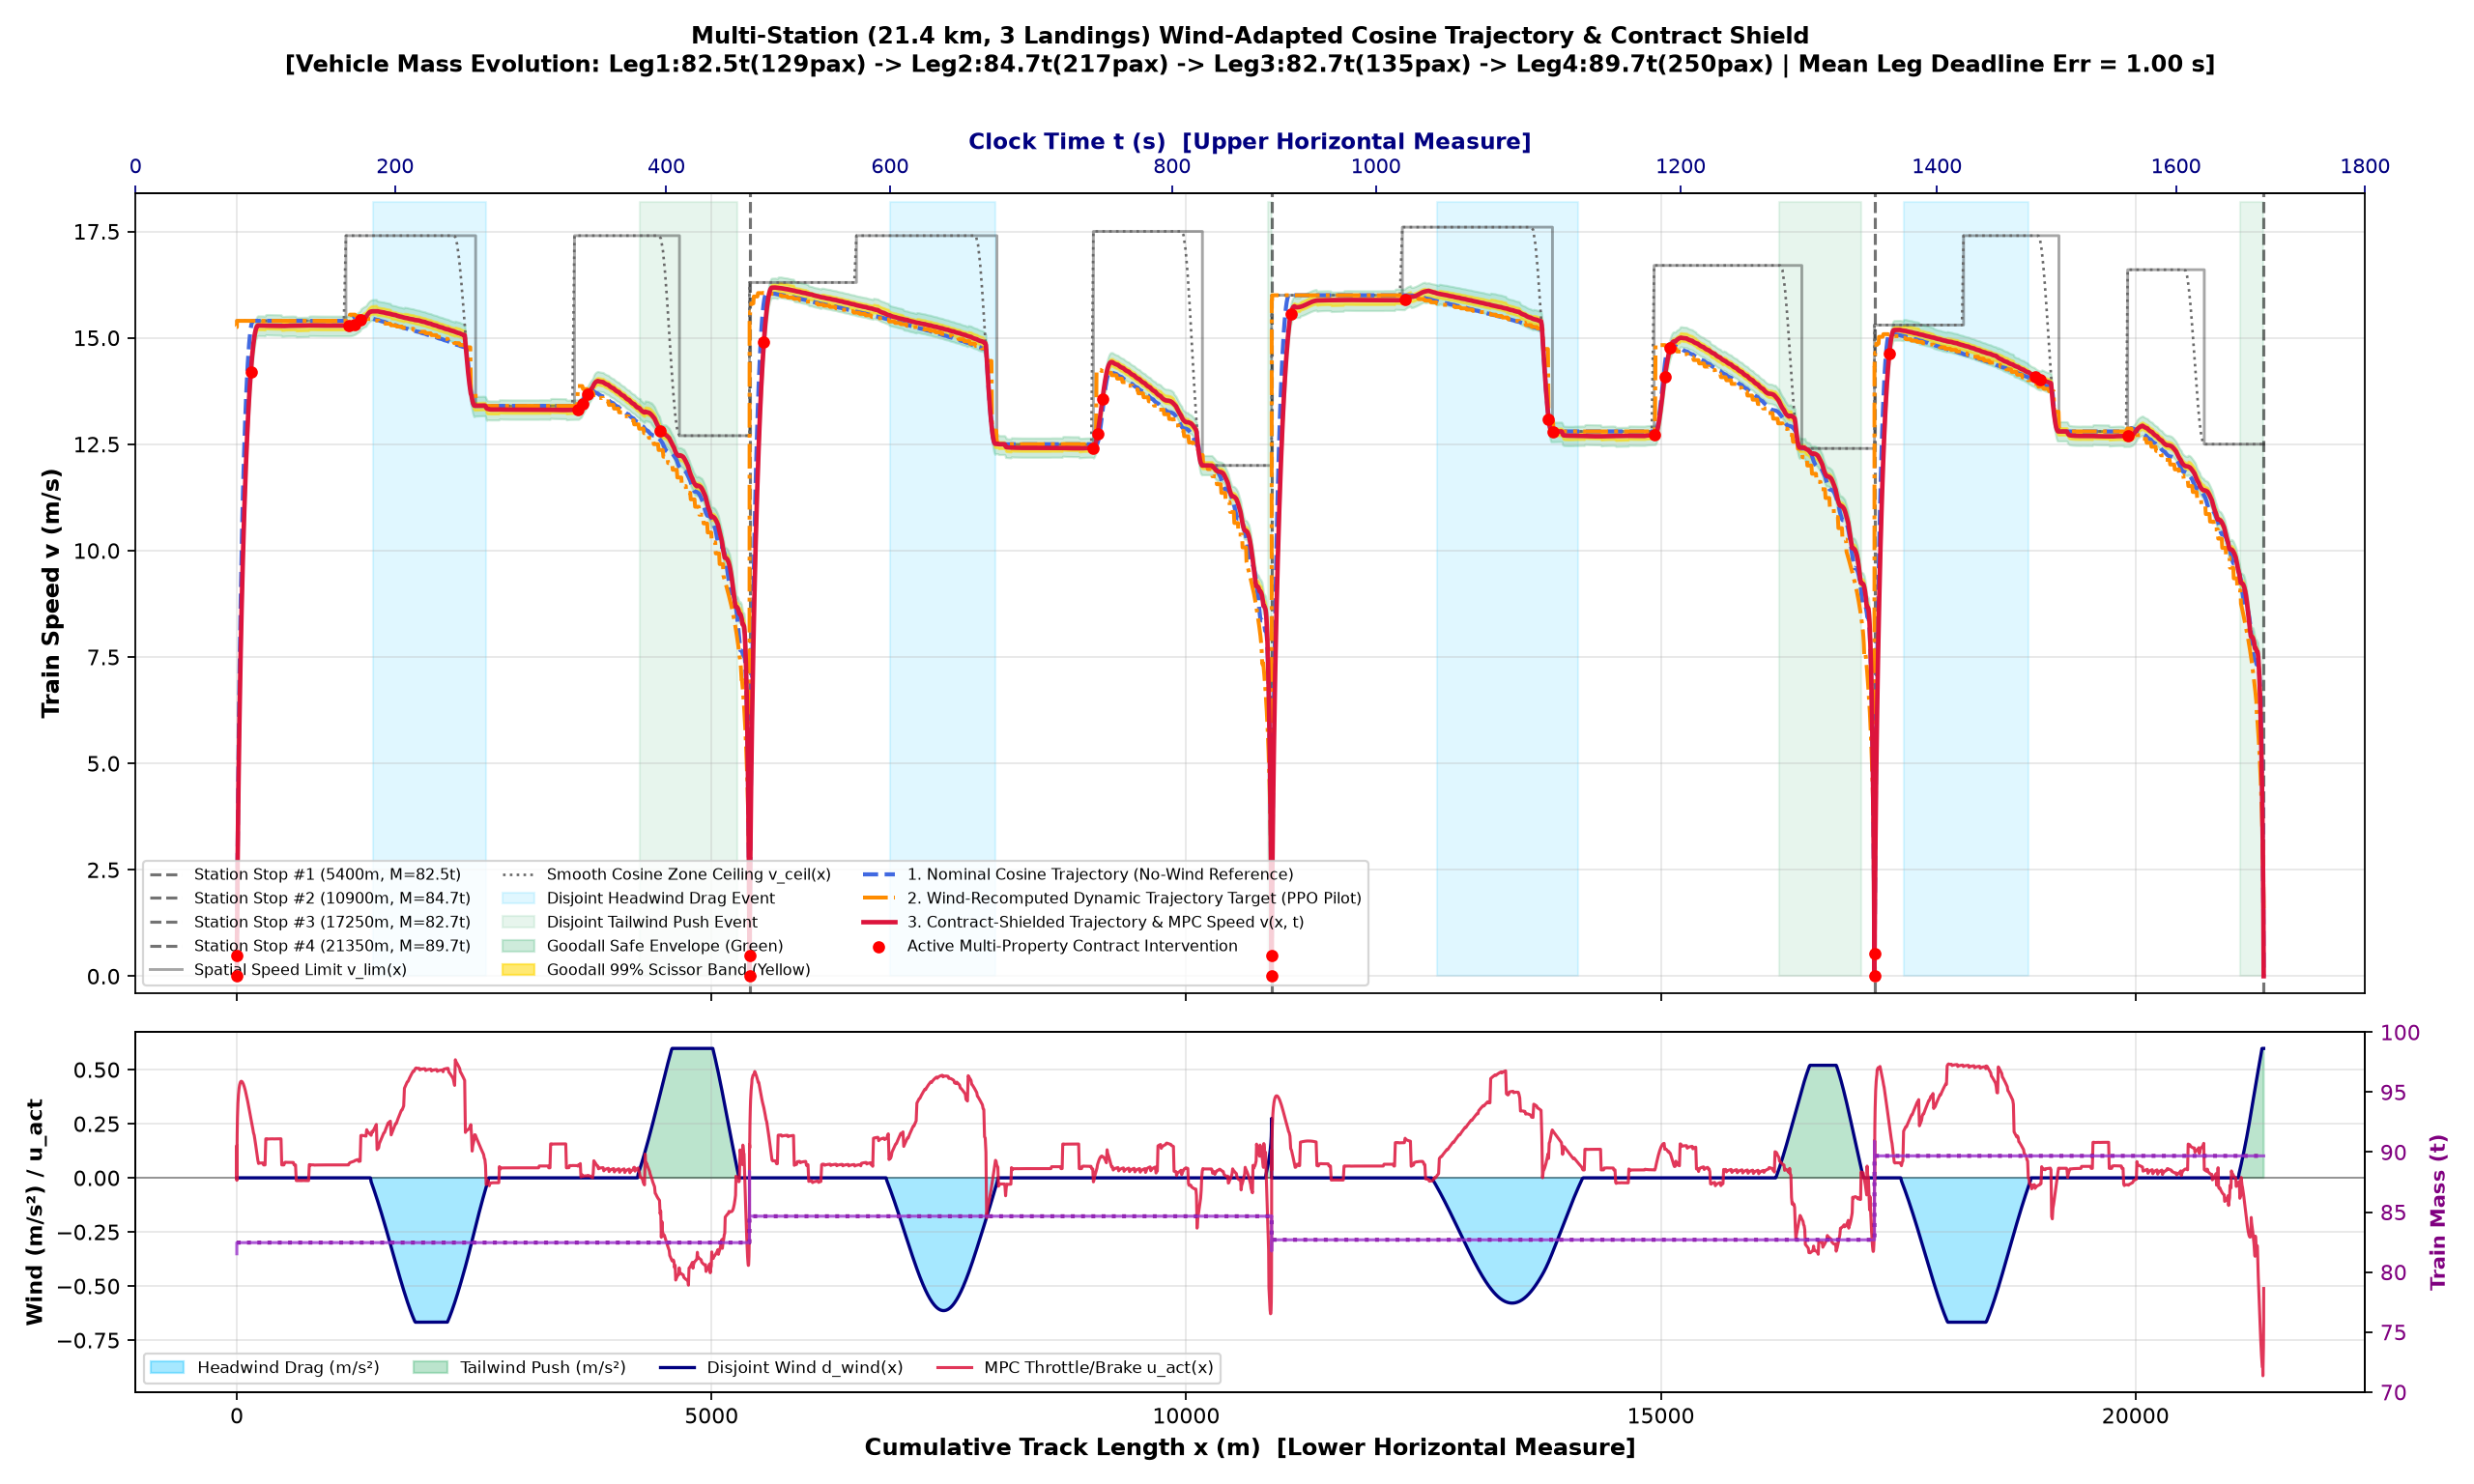
\includegraphics[width=0.91\textwidth]{wind_trajectory_shield_dual_axis.png}
\caption{Dual-horizontal-axis 4-station ($21.35\text{ km}$) evaluation showing cumulative track length $x$ (m) on the lower horizontal axis and clock time $t$ (s) on the upper horizontal axis. Top: Nominal no-wind trajectory (blue dashed), wind-recomputed PPO target (orange dash-dot), and Contract-Shielded MPC velocity (red solid) inside the Goodall 99\% Scissor Band (yellow) and Safe Envelope (green). Bottom: Headwind and tailwind events, MPC actuator effort $u_{\text{act}}$, and the 8-step identified passenger mass $\hat{M}(x)$ converging onto the true train mass $M(x)$.}
\label{fig:dual_axis}
\end{figure}

\begin{figure}[H]
\centering
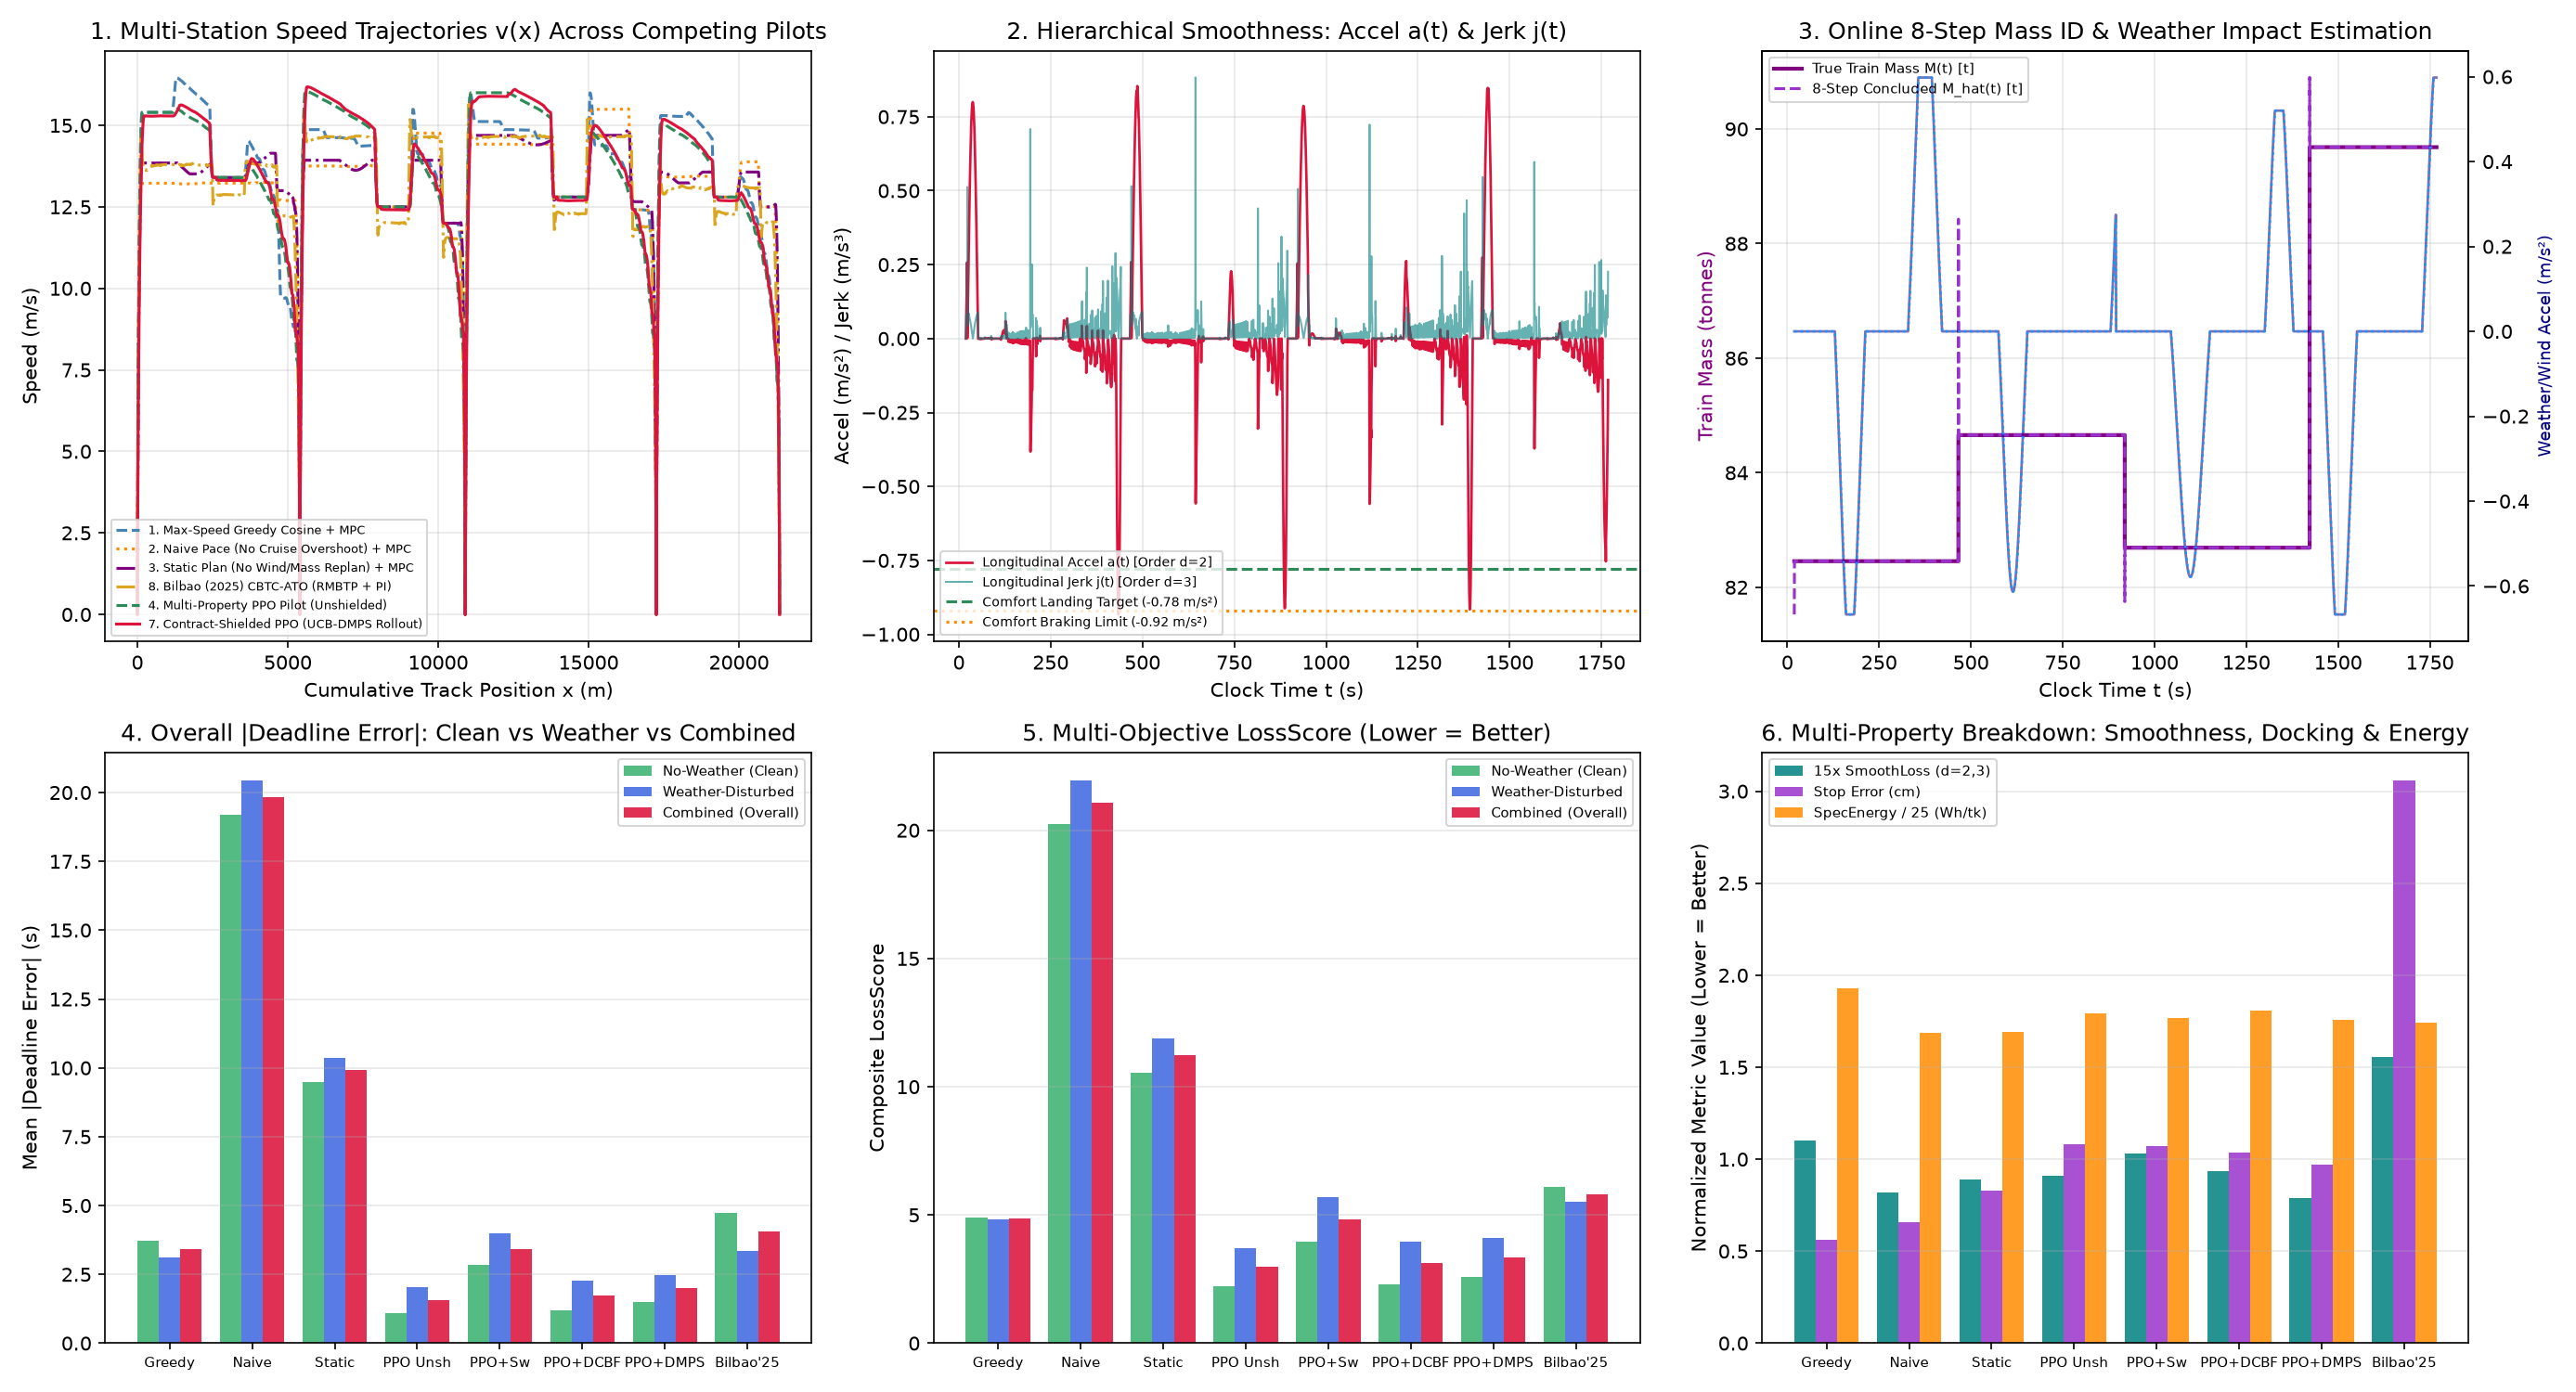
\includegraphics[width=0.95\textwidth]{rl_cosine_mpc.png}
\caption{Six-panel benchmark overview across all eight competing controllers: (1) multi-station speed profiles $v(x)$, (2) Order-2 acceleration $a(t)$ and Order-3 jerk $j(t)$, (3) online 8-step passenger mass identification and weather observer $\hat{d}(t)$, (4) mean deadline error across Clean, Weather-Disturbed, and Combined runs, (5) composite multi-objective LossScore, and (6) normalized breakdown of $15\times\text{SmoothLoss}$, Stop Error (cm), and $\text{SpecEnergy}/25$ (Wh/t-km).}
\label{fig:six_panel}
\end{figure}

\FloatBarrier
\section{Conclusions}

The three-stage control architecture developed in this work demonstrates how low-level actuator physics, online disturbance estimation, and high-level multi-property trajectory planning can be unified within a single real-time framework. In Stage 1, lifting the first-order motor delay directly into a state-augmented LTV-MPC eliminated ramp-termination overshoot and enabled a learned heteroscedastic scissor tube to replace offline polyhedral reachability sets. In Stage 2, compressing the prediction horizon to $N_p = 5, N_c = 3$ and introducing a gust-gated disturbance observer halved tracking error under storm bursts. In Stage 3, combining 8-step station departure mass identification with a macro-step PPO trajectory pilot, a phase-tracked $C^2$ half-cosine shaper, and a hierarchical Assume-Guarantee contract shield extended the controller to multi-station deadline-driven operation \cite{zhong2022,xiao2023}.

Evaluating candidate ramps at initiation and latching gentler backup contracts ($\mathcal{C}_2, \mathcal{C}_4$) across the ramp duration with $+0.06\text{ m/s}$ cruise compensation allows the contract shield to reduce $\text{SmoothLoss}$ by up to $17.7\%$ (from $0.0606$ down to $0.0499$ in Switch MPS, $0.0519$ in 1-Step DCBF, and $0.0527$ in UCB-DMPS Rollout, over $50\%$ lower than Bilbao-Moreno et al.\ \cite{bilbao2025}) while saving up to $0.86\text{ Wh/t-km}$ of traction energy and intervening on only $7.7\%\text{--}8.9\%$ of macro-steps. Finally, replacing generic matrix routines and per-step tensor dispatch with upper-triangular scalar recurrence, a closed-form $3\times 3$ Cramer QP solver, smooth unclamped Taylor linearization, lazy 2-step rollout verification, and zero-copy in-place NumPy parameter views yields a core shaper-plus-MPC step time of $10.7\text{--}11.4\text{ }\mu\text{s}$ (nearly $2\times$ faster than the $19.9\text{ }\mu\text{s}$ CBTC-ATO cascade PI baseline \cite{bilbao2025}) and a total shielded control cycle of $22.7\text{--}23.5\text{ }\mu\text{s}$ mean ($40.0\text{--}42.7\text{ }\mu\text{s}$ P99) with $1.0\text{ cm}$ station stopping accuracy and $99.96\%$ physical tube containment across all 30 scenarios.

\begin{thebibliography}{99}
\footnotesize
\bibitem{havaei2022} P. Havaei and M. A. Sandidzadeh, ``Intelligent-PID controller design for speed track in automatic train operation system with heuristic algorithms,'' \textit{Journal of Rail Transport Planning \& Management}, vol. 22, p. 100321, 2022.
\bibitem{liu2025} D. Liu, G. Yan, J. Zhou, and B. Chen, ``MPC-Based Speed Tracking Control for Subway Trains Under Actuator Constraints,'' \textit{Actuators}, vol. 14, no. 3, p. 134, 2025.
\bibitem{banerjee2024} A. Banerjee, K. Rahmani, J. Biswas, and I. Dillig, ``Dynamic Model Predictive Shielding for Provably Safe Reinforcement Learning,'' \textit{arXiv preprint arXiv:2405.13863}, 2024.
\bibitem{goodall2026} A. W. Goodall and F. Belardinelli, ``Safe Reinforcement Learning via Recovery-based Shielding with Gaussian Process Dynamics Models,'' in \textit{Proc. 25th Int. Conf. on Autonomous Agents and Multiagent Systems (AAMAS)}, 2026, pp. 540--549.
\bibitem{goodall_code} A. W. Goodall, ``A2C-GP-Shield: Official Implementation of Safe Reinforcement Learning via Recovery-based Shielding with Gaussian Process Dynamics Models,'' GitHub Repository, 2026.
\bibitem{hsu2024} K.-C. Hsu, H. Hu, and J. F. Fisac, ``The Safety Filter: A Unified View of Safety-Critical Control in Autonomous Systems,'' \textit{Annual Review of Control, Robotics, and Autonomous Systems}, vol. 7, pp. 47--72, 2024.
\bibitem{wang2023} Y. Wang et al., ``Enforcing Hard Constraints with Soft Barriers: Safe Reinforcement Learning in Unknown Stochastic Environments,'' in \textit{Proc. 40th Int. Conf. on Machine Learning (ICML)}, PMLR, vol. 202, 2023, pp. 36593--36604.
\bibitem{cannon2010} M. Cannon, B. Kouvaritakis, and X. Wu, ``Model predictive control for systems with stochastic disturbances and uncertain dynamics,'' \textit{Automatica}, vol. 46, no. 6, pp. 1195--1204, 2010.
\bibitem{mayne2005} D. Q. Mayne, M. M. Seron, and S. V. Rakovi\'{c}, ``Robust model predictive control of constrained linear systems with bounded disturbances,'' \textit{Automatica}, vol. 41, no. 2, pp. 219--224, 2005.
\bibitem{cano2026} F. Cano, T. A. Henzinger, and K. Kueffner, ``Shielding for Higher-Order Safety,'' \textit{arXiv preprint arXiv:2608.03662v1}, Aug. 2026.
\bibitem{adalat2026a} O. Adalat, E. Hamel-De le Court, and F. Belardinelli, ``Contract-Based Compositional Shielding for Safe Multi-Agent Reinforcement Learning,'' \textit{arXiv preprint arXiv:2606.14130v2}, Jul. 2026.
\bibitem{adalat2026b} O. Adalat, E. Hamel-De le Court, and F. Belardinelli, ``Contract-enabled Communication for Safe Multi-Agent Reinforcement Learning,'' in \textit{Proc. 26th Int. Conf. on Autonomous Agents and Multiagent Systems (AAMAS)}, 2027.
\bibitem{agarwal2021} A. Agarwal, S. M. Kakade, J. D. Lee, and G. Mahajan, ``On the Theory of Policy Gradient Methods: Optimality, Approximation, and Distribution Shift,'' \textit{Journal of Machine Learning Research (JMLR)}, vol. 22, no. 98, pp. 1--76, 2021.
\bibitem{mei2020} J. Mei, C. Xiao, C. Szepesv\'{a}ri, and D. Schuurmans, ``On the Global Convergence Rates of Softmax Policy Gradient Methods,'' in \textit{Proc. 37th Int. Conf. on Machine Learning (ICML)}, PMLR, vol. 119, 2020, pp. 6820--6829.
\bibitem{zhong2022} W. Zhong, S. Li, H. Xu, and W. Zhang, ``On-line train speed profile generation of high-speed railway with energy-saving: A model predictive control method,'' \textit{IEEE Transactions on Intelligent Transportation Systems}, vol. 23, no. 5, pp. 4063--4074, May 2022.
\bibitem{xiao2023} Z. Xiao, N. Murgovski, M. Chen, X. Feng, Q. Wang, and P. Sun, ``Eco-driving for metro trains: A computationally efficient approach using convex programming,'' \textit{IEEE Transactions on Vehicular Technology}, vol. 72, no. 8, pp. 10063--10076, Aug. 2023.
\bibitem{bilbao2025} A. Bilbao-Moreno, I. Elorza, E. Irigoyen, and I. Trojaola, ``ATO system for CBTC-based railways: Planning and disturbance estimation for enhanced automation,'' \textit{Results in Engineering}, vol. 26, p. 105357, 2025.
\bibitem{sun2024} P. Sun, J. Zhang, K. Yan, B. Yao, and Q. Wang, ``Event-triggered tube model predictive control for high-speed trains trajectory tracking based on robust reachable set,'' in \textit{Proc. SPIE 13064, 3rd Int. Conf. on Electronic Information Engineering, Big Data, and Computer Technology (EIBDCT)}, p. 130640F, 2024.
\end{thebibliography}

\end{document}
